\documentclass{beamer}
\mode<presentation>
{
  \usetheme{default}
  \useinnertheme{circles}
  \usenavigationsymbolstemplate{} % no navigation symbols
  \setbeamercovered{transparent}
}

\usepackage[english]{babel}
\usepackage[latin1]{inputenc}
\usepackage{times}
\usepackage[T1]{fontenc}
\usepackage{listings}

\setbeamertemplate
{footline}
{\hfill\insertframenumber/\inserttotalframenumber\quad\insertsection}
%{\quad\strut\insertsection\hfill\insertframenumber/\inserttotalframenumber
%\strut\quad}

\usepackage{pgfpages}
%\pgfpagesuselayout{2 on 1}[letterpaper,border shrink=20mm]
\pgfpagesuselayout{resize to}[letterpaper,border shrink=5mm,landscape]

%%%%%%%%%%%%%%%%%%%%%%%%%%%%%%%%%%%%%%%%%%%%%%%%%%%%%%%%%%%%%%%%%%%%%
% header
%%%%%%%%%%%%%%%%%%%%%%%%%%%%%%%%%%%%%%%%%%%%%%%%%%%%%%%%%%%%%%%%%%%%%


\title
{Nauty \\
A Brief Introduction}

\author[caw rit]
{Christopher A. Wood\\
{\small Department of Computer Science}\\
{\small Rochester Institute of Technology}\\
{\small\tt caw4567@cs.rit.edu}}

\date[CSC 2010] % (optional, should be abbreviation of conference name)
%{CSC@RIT, 29 Jan 2010}
%{TC@URCS, 1 Feb 2010}
%{math@WVU, 2 Mar 2010}
{RIT Folkman Group\\ \today}

\pgfdeclareimage[height=0.5cm]{university-logo}{logo.jpg}
\logo{\pgfuseimage{university-logo}}

%%%%%%%%%%%%%%%%%%%%%%%%%%%%%%%%%%%%%%%%%%%%%%%%%%%%%%%%%%%%%%%%%%%%%

\begin{document}

\begin{frame}
  \titlepage
\end{frame}

%%%%%%%%%%%%%%%%%%%%%%%%%%%%%%%%%%%%%%%%%%%%%%%%%%%%%%%%%%%%%%%%%%%%%

\begin{frame}{Nauty}
{main functionality}

A \textbf{graph canonical labeling} program with two main purposes

\bigskip
\begin{itemize}
\item
determine the automorphism group of a vertex-colored graph (\textbf{nauty} = no automorphisms, yes?)
\item
generate non-isomorphic graphs
\end{itemize}

\end{frame}

%%%%%%%%%%%%%%%%%%%%%%%%%%%%%%%%%%%%%%%%%%%%%%%%%%%%%%%%%%%%%%%%%%%%%

\begin{frame}{Graph automorphism}
{definition}

\emph{Graph automorphism}: A vertex mapping that preserves connectivity between vertex and edge
connectivity (e.g. an isomorphism onto itself)

\medskip

The set of all automorphism on a graph is the \emph{automorphism group}

\medskip

\begin{center}
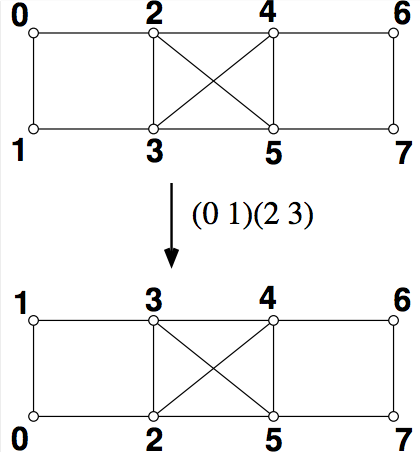
\includegraphics[scale=0.3]{automorphism.png} 
\end{center}
{\small [McKay]}

\end{frame}

%%%%%%%%%%%%%%%%%%%%%%%%%%%%%%%%%%%%%%%%%%%%%%%%%%%%%%%%%%%%%%%%%%%%%

\begin{frame}{Graph isomorphism}
{definition}

\emph{Graph isomorphism}: A vertex mapping that $f : V(G) \to V(H)$ such that if $(u,v) \in E(G)$ then $(f(u), f(v)) \in E(H)$.

\medskip
\begin{itemize}
\item
The \emph{canonical labeling} feature of nauty reduces all isomorphic graphs down to the same identical graph. 
\item
This is how nonisomorphic graphs are found!
\end{itemize}

\end{frame}

%%%%%%%%%%%%%%%%%%%%%%%%%%%%%%%%%%%%%%%%%%%%%%%%%%%%%%%%%%%%%%%%%%%%%

\begin{frame}{Graph isomorphism}
{finding isomorphic graphs through canonization}

\begin{center}
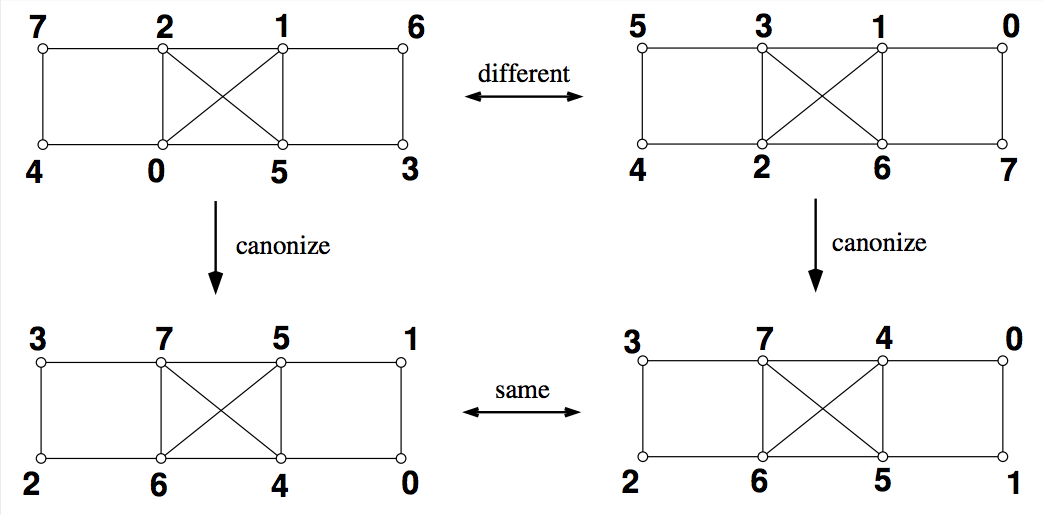
\includegraphics[scale=0.3]{canonical.png}
\end{center}
{\small [McKay]}

\end{frame}

%%%%%%%%%%%%%%%%%%%%%%%%%%%%%%%%%%%%%%%%%%%%%%%%%%%%%%%%%%%%%%%%%%%%%

\begin{frame}[fragile] {Using nauty}
{getting started with dreadnaut}

Nauty (and Traces) can be downloaded at:
{\tt http://pallini.di.uniroma1.it} 

\bigskip

Getting started (see what commands are available)... 

\bigskip

\begin{lstlisting}[frame=single]
raven-2:nauty caw$ dreadnaut
Dreadnaut version 2.4 (64 bits).
> h 
\end{lstlisting}

\end{frame}

%%%%%%%%%%%%%%%%%%%%%%%%%%%%%%%%%%%%%%%%%%%%%%%%%%%%%%%%%%%%%%%%%%%%%

\begin{frame}[fragile] {Using nauty}
{a short example}

\begin{center}
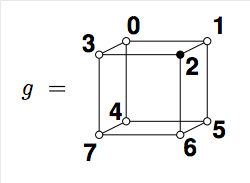
\includegraphics[scale=0.3]{dreadnautExample.png}
\end{center}

\bigskip

\begin{lstlisting}[frame=single]
> n=8 g
> 0: 1 3 4; enter the graph
  1: 2 5;
  2: 3 6;
  3: 7;
  4: 5 7;
  5: 6;
  6: 7. 
> f=2 x
[fixing partition]
\end{lstlisting}
[McKay]

\end{frame}

%%%%%%%%%%%%%%%%%%%%%%%%%%%%%%%%%%%%%%%%%%%%%%%%%%%%%%%%%%%%%%%%%%%%%

\begin{frame}[fragile] {Scaling up}
{size limits}

Nauty is limited by the word size $n$ of the machine on which it is compiled (unfortunately)

\bigskip

\begin{itemize}
\item 
$n < 32$ {\tt int} $\to 2^{15} - 3$ limit
\item 
$n \leq 32$ {\tt int} $\to 2^{30}$ limit
\end{itemize}

These are limits on the number of vertices (the order of the graph)

\end{frame}

%%%%%%%%%%%%%%%%%%%%%%%%%%%%%%%%%%%%%%%%%%%%%%%%%%%%%%%%%%%%%%%%%%%%%

\begin{frame}[fragile] {Wrapping nauty}
{writing our own code}

We can easily use nauty procedures internally:

\bigskip

\begin{enumerate}
\item 
Include {\tt nauty.h} and link to {\tt nauty.c}, {\tt nautil.c}, {\tt naugraph.c}, {\tt schreier.c}, and {\tt naurng.c}.
\item 
Use any of the functions and macros defined in {\tt nauty.h}!
\end{enumerate}

\begin{lstlisting}[frame=single]
#define MAXN 1000 
#define MAXM 1000 
#include "nauty.h" 
int main(int argc, char *argv[]) {
   graph g[MAXN*MAXM];
   // your code goes here...
\end{lstlisting}
[McKay]

\end{frame}

%%%%%%%%%%%%%%%%%%%%%%%%%%%%%%%%%%%%%%%%%%%%%%%%%%%%%%%%%%%%%%%%%%%%%

\begin{frame}[fragile] {Useful utilities}
{automatic graph manipulation without writing your own code}

\bigskip

\begin{itemize}
\item 
\textbf{geng} : generate small graphs
\item 
\textbf{genbg} : generate small bicoloured graphs
\item 
\textbf{gentourng} : generate small tournaments
\item 
\textbf{directg} : generate small digraphs with given underlying graph
\item 
\textbf{watercluster2} : a faster alternative to direct written by Gunnar Brinkmann
\item 
\textbf{multig} : generate small multigraphs with given underlying graph
\item 
\textbf{genrang} : generate random graphs
\item 
\textbf{copyg} : convert format and select subset
\item 
\textbf{labelg} : canonically label graphs
\end{itemize}

\end{frame}

%%%%%%%%%%%%%%%%%%%%%%%%%%%%%%%%%%%%%%%%%%%%%%%%%%%%%%%%%%%%%%%%%%%%%

\begin{frame}[fragile] {What else?}
{}

Consult the manual! :-)

\end{frame}

%%%%%%%%%%%%%%%%%%%%%%%%%%%%%%%%%%%%%%%%%%%%%%%%%%%%%%%%%%%%%%%%%%%%%

\begin{frame}{References}

\begin{itemize}
\item
McKay, Brendan D., and Adolfo Piperno. \emph{nauty and Traces User's Guide (Version 2.5).} 2013.
\end{itemize}
\end{frame}

%%%%%%%%%%%%%%%%%%%%%%%%%%%%%%%%%%%%%%%%%%%%%%%%%%%%%%%%%%%%%%%%%%%%%

\end{document}
